\section{QCD AND HADRON STRUCTURE}
\label{sec:qcd_hadron}

This chapter collects the theoretical background for the rest of the thesis. We start with conventions and with the path integral formulation of quantum field theory, which is the starting point of lattice QCD. We then introduce QCD, its gauge symmetry and the Wilson lines that make non-local operators gauge invariant, and we review asymptotic freedom and confinement. The second half of the chapter turns to hadron structure. We describe deep inelastic scattering and the collinear parton distributions, then semi-inclusive DIS and the Drell-Yan process, which lead to transverse momentum dependent distributions. We define TMDs with process-dependent gauge links, explain why the Sivers function changes sign between SIDIS and Drell-Yan, discuss rapidity divergences and the soft factor, and introduce the generalized Sivers shift computed in this work. The chapter ends with an overview of how TMDs can be accessed in lattice QCD. The detailed parametrization used in our calculation is given in Chapter~\ref{sec:tmd_framework}, and the lattice methods in Chapter~\ref{sec:lattice_methodology}.

\subsection{Conventions}
\label{sec:conventions}

We use natural units, $\hbar = c = 1$, and the Minkowski metric $g^{\mu\nu} = \mathrm{diag}(+1,-1,-1,-1)$. Light-cone components of a four-vector $w$ are defined by
\begin{equation}
  w^{\pm} = \frac{1}{\sqrt{2}}\left(w^0 \pm w^3\right) ,
  \label{eq:lightcone_components}
\end{equation}
and we write $w = (w^+, w^-, \vprp{w})$, where the bold transverse vector $\vprp{w} = (w^1,w^2)$ is a Euclidean two-vector. Scalar products read
\begin{equation}
  a\tcdot b = a^+ b^- + a^- b^+ - \vprp{a}\tcdot\vprp{b} \ .
\end{equation}
It is convenient to introduce the light-like vectors $\nplus = (1,0,0,1)/\sqrt{2}$ and $\nminus = (1,0,0,-1)/\sqrt{2}$, which satisfy $\nplus^2 = \nminus^2 = 0$ and $\nplus\tcdot\nminus = 1$, so that $w^+ = \nminus\tcdot w$ and $w^- = \nplus\tcdot w$. A nucleon of mass $\mN$ moving along the positive $z$ axis with no transverse momentum has
\begin{equation}
  P = P^+\,\nplus + \frac{\mN^2}{2P^+}\,\nminus \ ,
\end{equation}
and its spin vector is
\begin{equation}
  S = \Lambda\,\frac{P^+}{\mN}\,\nplus - \Lambda\,\frac{\mN}{2P^+}\,\nminus + \vprp{S} \ ,
\end{equation}
where $\Lambda$ is the helicity and $\vprp{S}$ the transverse spin, with $\Lambda^2 + \vprp{S}^2 = 1$ for a pure state. The Levi-Civita tensor is normalized as $\epsilon^{0123} = +1$, and the transverse tensor $\epsilon_{ij}\equiv\epsilon_{-+ij}$ has $\epsilon_{12} = +1$. We use $\gamma^{\pm} = (\gamma^0\pm\gamma^3)/\sqrt{2}$, $\gamma_5 = i\gamma^0\gamma^1\gamma^2\gamma^3$ and $\sigma^{\mu\nu} = \frac{i}{2}[\gamma^\mu,\gamma^\nu]$. Nucleon states are normalized covariantly, $\langle P',S'|P,S\rangle = 2E_P\,(2\pi)^3\delta^{3}(\vect{P}-\vect{P}')\,\delta_{SS'}$. These conventions follow Ref.~\cite{Musch:2011er}. The relations between Minkowski and Euclidean gamma matrices used in the lattice analysis are listed in Section~\ref{sec:solving_amplitudes}.

In this convention a parton with light-cone momentum fraction $x$ has $k^+ = xP^+$. Some references, including the TMD Handbook \cite{Boussarie:2023izj}, place the antiquark field at $\bvec$ and the quark field at the origin, which reverses the sign of $\bvec$ relative to our definitions. We always write the operator as $\bar{q}(0)\,\Gamma\,\mathcal{U}\,q(\bvec)$, as in Refs.~\cite{Musch:2010ka,Musch:2011er}.

\subsection{Quantum field theory and the path integral}
\label{sec:path_integral}

A quantum field theory is fully specified by its correlation functions, the vacuum expectation values of time-ordered products of field operators. For a scalar field $\phi$ with action $S[\phi] = \int d^4x\, \mathcal{L}(\phi,\partial\phi)$, the path integral expresses them as \cite{Peskin:1995ev}
\begin{equation}
  \langle\Omega|\,T\{\phi(x_1)\cdots\phi(x_n)\}\,|\Omega\rangle
  = \frac{\int\mathcal{D}\phi\ \phi(x_1)\cdots\phi(x_n)\ e^{iS[\phi]}}{\int\mathcal{D}\phi\ e^{iS[\phi]}} \ .
  \label{eq:minkowski_pi}
\end{equation}
The oscillating weight $e^{iS}$ makes this expression hard to define and unsuitable for numerical evaluation. Both problems are removed by a rotation to imaginary time. Setting $x^0 = -i x_4$ with real $x_4$, the action turns into $iS \to -S_E$, where $S_E$ is the Euclidean action, and correlation functions become
\begin{equation}
  \langle \mathcal{O}_1\cdots\mathcal{O}_n\rangle_E = \frac{1}{Z}\int\mathcal{D}\phi\ \mathcal{O}_1\cdots\mathcal{O}_n\ e^{-S_E[\phi]}\ ,
  \qquad Z = \int\mathcal{D}\phi\ e^{-S_E[\phi]} \ .
  \label{eq:euclidean_pi}
\end{equation}
For a bosonic theory with a real, bounded-below action, $e^{-S_E}/Z$ is a probability distribution over field configurations. This is what allows Monte Carlo methods to be used once space-time is discretized, as described in Chapter~\ref{sec:lattice_methodology}.

The Euclidean formulation has a simple connection to the spectrum of the Hamiltonian $H$. For an operator $\mathcal{O}$ with Euclidean time dependence $\mathcal{O}(\tau) = e^{H\tau}\mathcal{O}(0)e^{-H\tau}$, inserting a complete set of energy eigenstates gives
\begin{equation}
  \langle\Omega|\,\mathcal{O}(\tau)\,\mathcal{O}^\dagger(0)\,|\Omega\rangle = \sum_n \big|\langle\Omega|\mathcal{O}|n\rangle\big|^2\, e^{-(E_n - E_\Omega)\tau} \ .
  \label{eq:spectral_decomposition}
\end{equation}
At large Euclidean time, the lowest state with nonzero overlap dominates. Hadron masses and matrix elements are extracted from lattice correlation functions in exactly this way (Chapter~\ref{sec:lattice_methodology}).

Fermions are described by anticommuting Grassmann fields $\psi$ and $\bar{\psi}$. For an action bilinear in the fermion fields, $S_F = \int d^4x\,\bar{\psi}\,M\,\psi$, the Grassmann integral can be done exactly,
\begin{equation}
  \int\mathcal{D}\bar\psi\,\mathcal{D}\psi\ e^{-\bar\psi M\psi} = \det M \ ,
  \qquad
  \langle\psi(x)\,\bar\psi(y)\rangle = M^{-1}(x,y) \ .
  \label{eq:grassmann}
\end{equation}
In QCD, $M$ is the Dirac operator in a background gluon field, so integrating out the quarks leaves a path integral over gluon fields only, weighted by $\det M$ times the exponential of the gauge action. Correlation functions of quark operators become products of quark propagators $M^{-1}$ averaged over gluon configurations.

\subsection{Gauge invariance and QCD}
\label{sec:qcd_lagrangian}

QCD is a non-Abelian gauge theory with gauge group $SU(3)$ \cite{Yang:1954ek,Fritzsch:1973pi,Gross:1973id,Politzer:1973fx}. Each quark flavor $f$ is a Dirac spinor carrying a color index in the fundamental representation. The gluon field $A_\mu = A^a_\mu t^a$ takes values in the Lie algebra, where the generators $t^a = \lambda^a/2$, $a=1,\dots,8$, are built from the Gell-Mann matrices $\lambda^a$ and satisfy
\begin{equation}
  [t^a, t^b] = i f^{abc}\, t^c \ ,\qquad \mathrm{tr}\left(t^a t^b\right) = \frac{1}{2}\delta^{ab} \ ,
\end{equation}
with the $SU(3)$ structure constants $f^{abc}$. The QCD Lagrangian density is
\begin{equation}
  \mathcal{L}_{\text{QCD}} = \sum_{f} \bar{q}_f(x)\left(i\gamma^\mu D_\mu - m_f\right) q_f(x) - \frac{1}{4} F^a_{\mu\nu}(x) F^{a\,\mu\nu}(x) \ ,
  \label{eq:qcd_lagrangian}
\end{equation}
with the covariant derivative and field strength tensor
\begin{align}
  D_\mu &= \partial_\mu - i g\, A^a_\mu\, t^a \ , \\
  F^a_{\mu\nu} &= \partial_\mu A^a_\nu - \partial_\nu A^a_\mu + g\, f^{abc} A^b_\mu A^c_\nu \ .
\end{align}
Here $g$ is the gauge coupling and $m_f$ the quark mass of flavor $f$. The last term in $F^a_{\mu\nu}$ makes the gluons interact with each other. The photon of quantum electrodynamics carries no charge and has no such self-interaction.

The Lagrangian is invariant under local $SU(3)$ transformations $V(x) = \exp\left(i\alpha^a(x)t^a\right)$,
\begin{align}
  q(x) &\to V(x)\,q(x)\ , \qquad \bar{q}(x) \to \bar{q}(x)\,V^\dagger(x)\ , \nonumber\\
  A_\mu(x) &\to V(x)A_\mu(x)V^\dagger(x) - \frac{i}{g}\big(\partial_\mu V(x)\big)V^\dagger(x) \ ,
  \label{eq:gauge_transformation}
\end{align}
under which $D_\mu q \to V D_\mu q$ and $F_{\mu\nu} \to V F_{\mu\nu} V^\dagger$. Physical observables must be gauge invariant.

Gauge invariance has an immediate consequence for the operators that define parton distributions. A local bilinear such as $\bar{q}(x)\Gamma q(x)$ is gauge invariant, but a non-local bilinear $\bar{q}(x)\Gamma q(y)$ with $x\neq y$ is not, because the two fields transform with $V$ at different points. The fields have to be connected by a Wilson line, the parallel transporter of color along a path. For a path $\mathcal{C}$ that starts at $x$ and ends at $y$ we define
\begin{equation}
  \mathcal{U}[\mathcal{C}] = \mathcal{P}\exp\left(-i g \int_{\mathcal{C}} dz^\mu\, A_\mu(z)\right) ,
  \label{eq:wilson_line}
\end{equation}
where the path ordering $\mathcal{P}$ places fields at points closer to the start of the path to the left. This Wilson line transforms as
\begin{equation}
  \mathcal{U}[\mathcal{C}] \to V(x)\,\mathcal{U}[\mathcal{C}]\,V^\dagger(y) \ ,
\end{equation}
so the operator
\begin{equation}
  \bar{q}(x)\,\Gamma\,\mathcal{U}[\mathcal{C}]\,q(y)
  \label{eq:nonlocal_operator}
\end{equation}
is gauge invariant for any path from $x$ to $y$ and any Dirac matrix $\Gamma$. For a path made of straight segments through the points $x, z_1, \ldots, z_n, y$ we write $\Wline{x,z_1,\ldots,z_n,y} = \Wline{x,z_1}\,\Wline{z_1,z_2}\cdots\Wline{z_n,y}$, the notation used for the staple-shaped links in Eq.~\eqref{eq-staplelink}. The operator depends on the path, not only on the endpoints. Which path is appropriate cannot be decided by gauge invariance alone; for parton distributions it is fixed by the scattering process, as we explain in Section~\ref{sec:tmd_gauge_links}.

A Wilson line along a closed path is a Wilson loop, $W(\mathcal{C}) = \frac{1}{3}\mathrm{tr}\,\mathcal{U}[\mathcal{C}]$, which is gauge invariant by itself. Wilson loops are the basic objects of Wilson's lattice formulation \cite{Wilson:1974sk}. On the lattice, the gluon field is represented by link variables $U_\mu(x)$, which are the Wilson lines of single lattice links. The non-local operators of Eq.~\eqref{eq:nonlocal_operator} are then products of link variables along a path on the lattice, which makes them straightforward to evaluate.

The smallest Wilson loop on a lattice with spacing $a$ is the plaquette $U_{\mu\nu}(x)$, the product of the four links around an elementary square in the $\mu\nu$ plane. For small $a$ it can be written as $U_{\mu\nu}(x) = \exp\big(\pm i g a^2 F_{\mu\nu}(x) + \mathcal{O}(a^3)\big)$, with the sign fixed by the orientation of the loop, and expanding the exponential gives
\begin{equation}
  1 - \frac{1}{3}\,\mathrm{Re}\,\mathrm{tr}\,U_{\mu\nu}(x) = \frac{g^2 a^4}{6}\,\mathrm{tr}\big(F_{\mu\nu}(x)F_{\mu\nu}(x)\big) + \mathcal{O}(a^5) \qquad (\text{no sum over } \mu,\nu) \ .
  \label{eq:plaquette_expansion}
\end{equation}
Summing this expression over all plaquettes reproduces the Euclidean Yang-Mills action in the continuum limit. This is the origin of the Wilson gauge action used in Chapter~\ref{sec:lattice_methodology}.

\subsection{Asymptotic freedom, confinement and chiral symmetry}
\label{sec:af_confinement}

Quantum corrections make the QCD coupling depend on the momentum scale $\mu$ at which it is defined. With $\alpha_s = g^2/(4\pi)$, the renormalization group equation reads
\begin{equation}
  \mu^2\frac{d\alpha_s}{d\mu^2} = \beta(\alpha_s) = -\left(b_0\,\alpha_s^2 + b_1\,\alpha_s^3 + \cdots\right) ,
  \qquad b_0 = \frac{33 - 2n_f}{12\pi} \ ,
  \label{eq:beta_function}
\end{equation}
where $n_f$ is the number of quark flavors lighter than $\mu$. For $n_f \le 16$ the coefficient $b_0$ is positive, and at leading order
\begin{equation}
  \alpha_s(\mu^2) = \frac{1}{b_0\,\ln\left(\mu^2/\Lambda_{\text{QCD}}^2\right)} \ .
  \label{eq:running_coupling}
\end{equation}
The coupling decreases logarithmically at large $\mu$. This is asymptotic freedom \cite{Gross:1973id,Politzer:1973fx}, and it is why processes with a large momentum transfer can be computed in perturbation theory. At the $Z$ boson mass the coupling is $\alpha_s(M_Z) = 0.1180(9)$ \cite{ParticleDataGroup:2024cfk}. The scale $\Lambda_{\text{QCD}}$, a few hundred MeV, is generated dynamically; the classical Lagrangian with massless quarks contains no dimensionful parameter. As $\mu$ approaches $\Lambda_{\text{QCD}}$ the coupling becomes of order one and the perturbative expansion breaks down.

At long distances QCD confines color. No isolated quark or gluon has been observed, and the hadron spectrum consists of color-singlet states. On the lattice, confinement shows up as an area law for large Wilson loops. For a rectangular loop of spatial extent $R$ and temporal extent $T$,
\begin{equation}
  \langle W(R,T)\rangle \xrightarrow{T\to\infty} e^{-V(R)\,T} \ ,\qquad V(R) \approx \sigma R \quad (R\ \text{large}) \ ,
\end{equation}
where $V(R)$ is the potential between a static quark and antiquark and $\sigma$ is the string tension \cite{Wilson:1974sk,Creutz:1980zw}. The same kind of Wilson line self-interaction appears in the staple-shaped links of TMD operators, where it produces a dependence on the staple length that has to be removed by forming ratios (Section~\ref{sec:rapidity_soft}).

The third non-perturbative feature is the spontaneous breaking of chiral symmetry. For massless $u$ and $d$ quarks the Lagrangian is invariant under separate $SU(2)$ rotations of left- and right-handed quark fields. The QCD vacuum has a nonzero quark condensate $\langle\bar{q}q\rangle$, which breaks this symmetry down to the isospin subgroup. The pions are the corresponding pseudo-Goldstone bosons, light because the quark masses are small, and the Gell-Mann-Oakes-Renner relation $f_\pi^2 m_\pi^2 = -(m_u+m_d)\langle\bar{q}q\rangle$ links their mass to the condensate. Chiral symmetry breaking also explains why the nucleon, with a mass of about $0.94$~GeV, is much heavier than the sum of its valence quark masses. Its mass, like its internal structure, comes from the non-perturbative dynamics of QCD.

These three properties set the problem this thesis addresses. Asymptotic freedom makes hard scattering processes calculable, so that experiments can be interpreted in terms of parton distributions. Confinement and chiral symmetry breaking make the distributions themselves non-perturbative, so that computing them requires a method that does not rely on a small coupling. Lattice QCD is such a method.

\subsection{Deep inelastic scattering and the parton model}
\label{sec:dis}

In deep inelastic lepton-nucleon scattering, $\ell(l) + N(P) \to \ell(l') + X$, the lepton exchanges a virtual photon of momentum $q = l - l'$ with the nucleon, and the final hadronic state $X$ is not observed. The standard kinematic variables are
\begin{equation}
  Q^2 = -q^2 \ ,\qquad x_B = \frac{Q^2}{2P\tcdot q} \ ,\qquad y = \frac{P\tcdot q}{P\tcdot l} \ .
\end{equation}
The hadronic part of the cross section is contained in the hadronic tensor,
\begin{equation}
  W^{\mu\nu} = \frac{1}{4\pi}\int d^4\xi\ e^{iq\cdot\xi}\,\langle P|\,[J^\mu(\xi),J^\nu(0)]\,|P\rangle \ ,
\end{equation}
where $J^\mu$ is the electromagnetic current. Current conservation, parity and Lorentz invariance allow two structure functions for an unpolarized target,
\begin{equation}
  W^{\mu\nu} = \left(-g^{\mu\nu} + \frac{q^\mu q^\nu}{q^2}\right) F_1(x_B,Q^2)
  + \left(P^\mu - \frac{P\tcdot q}{q^2}\,q^\mu\right)\left(P^\nu - \frac{P\tcdot q}{q^2}\,q^\nu\right)\frac{F_2(x_B,Q^2)}{P\tcdot q} \ ,
\end{equation}
and, neglecting the nucleon mass, the cross section is
\begin{equation}
  \frac{d^2\sigma}{dx_B\,dQ^2} = \frac{4\pi\alpha^2}{x_B\,Q^4}\left[(1-y)\,F_2(x_B,Q^2) + x_B\,y^2\,F_1(x_B,Q^2)\right] .
\end{equation}

In the parton model the photon scatters elastically off a quark that carries a fraction $x$ of the nucleon's light-cone momentum. Momentum conservation at the photon vertex then sets $x = x_B$ up to corrections suppressed by $1/Q^2$, and the structure functions become
\begin{equation}
  F_2(x_B) = 2x_B F_1(x_B) = x_B\sum_q e_q^2\left[f_1^q(x_B) + f_1^{\bar q}(x_B)\right] ,
  \label{eq:parton_model_F2}
\end{equation}
where $e_q$ is the quark charge in units of the proton charge and $f_1^q(x)$ is the unpolarized PDF of quark flavor $q$ \cite{Feynman:1969ej,Bjorken:1968dy,Callan:1969uq}. The first equality, the Callan-Gross relation, reflects the spin $1/2$ of the quarks. The corresponding ``handbag'' diagram is shown in Figure~\ref{fig:handbag}.

\begin{figure}[htpb]
\centering
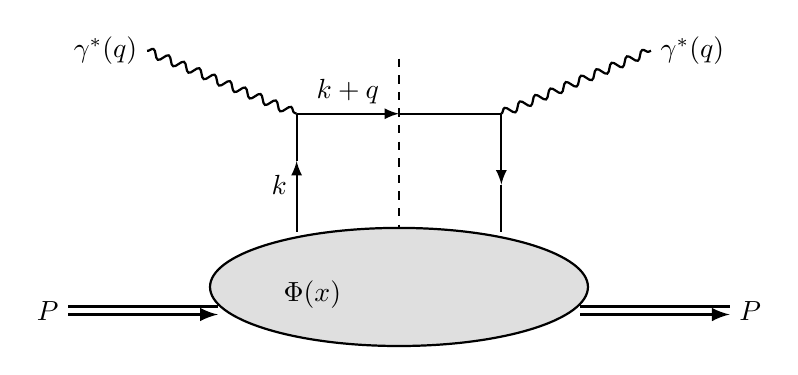
\begin{tikzpicture}[scale=1.0]
  % blob
  \filldraw[fill=gray!25, draw=black, thick] (0,0) ellipse (2.4 and 0.75);
  \node at (-1.1,-0.1) {$\Phi(x)$};
  % nucleon lines
  \draw[very thick, -latex] (-4.2,-0.35) -- (-2.3,-0.35);
  \draw[very thick] (-4.2,-0.25) -- (-2.3,-0.25);
  \node[left] at (-4.2,-0.3) {$P$};
  \draw[very thick, -latex] (2.3,-0.35) -- (4.2,-0.35);
  \draw[very thick] (2.3,-0.25) -- (4.2,-0.25);
  \node[right] at (4.2,-0.3) {$P$};
  % quark lines
  \draw[thick, -latex] (-1.3,0.7) -- (-1.3,1.6);
  \draw[thick] (-1.3,1.6) -- (-1.3,2.2);
  \draw[thick, -latex] (-1.3,2.2) -- (0,2.2);
  \draw[thick] (0,2.2) -- (1.3,2.2);
  \draw[thick, -latex] (1.3,2.2) -- (1.3,1.3);
  \draw[thick] (1.3,1.3) -- (1.3,0.7);
  \node[left] at (-1.3,1.3) {$k$};
  \node[above] at (-0.65,2.2) {$k+q$};
  % photons
  \draw[decorate, decoration={snake, amplitude=1.5pt, segment length=6pt}, thick] (-3.2,3.0) -- (-1.3,2.2);
  \draw[decorate, decoration={snake, amplitude=1.5pt, segment length=6pt}, thick] (1.3,2.2) -- (3.2,3.0);
  \node[left] at (-3.2,3.0) {$\gamma^*(q)$};
  \node[right] at (3.2,3.0) {$\gamma^*(q)$};
  % cut
  \draw[dashed] (0,2.9) -- (0,0.75);
\end{tikzpicture}
\caption{Handbag diagram for the leading contribution to the DIS hadronic tensor. The virtual photon scatters off a quark of momentum $k$ with $k^+ = xP^+$, and the lower blob is the quark-quark correlator whose $\gamma^+$ projection gives the PDF $f_1(x)$. The dashed line indicates the sum over final states.}
\label{fig:handbag}
\end{figure}

QCD turns the parton model into a controlled approximation. The collinear factorization theorem states that, up to power corrections in $1/Q$, the structure functions are convolutions of perturbatively calculable coefficient functions with PDFs defined as matrix elements of quark and gluon operators \cite{Collins:1981uw,CollinsBook2011}. For the unpolarized quark distribution this definition is
\begin{equation}
  f_1^q(x) = \frac{1}{2}\int\frac{db^-}{2\pi}\ e^{ixP^+ b^-}\,
  \langle P|\,\bar{q}(0)\,\gamma^+\,\Wline{0,\nminus b^-}\,q(\nminus b^-)\,|P\rangle \ .
  \label{eq:collinear_pdf}
\end{equation}
The quark fields are separated along the light-cone direction $\nminus$, and the straight Wilson line along $\nminus$ between them makes the operator gauge invariant. In light-cone gauge $A^+ = 0$ this Wilson line is equal to one, and $f_1^q(x)$ has the interpretation of a number density of quarks with plus-momentum $xP^+$ \cite{CollinsBook2011,Brodsky:1997de}. Eq.~\eqref{eq:collinear_pdf} has support on $-1\le x\le 1$. Positive $x$ corresponds to quarks, and negative $x$ to antiquarks, with $f_1^{\bar q}(x) = -f_1^q(-x)$ for $x>0$.

Replacing $\gamma^+$ in Eq.~\eqref{eq:collinear_pdf} by $\gamma^+\gamma_5$ or by $i\sigma^{i+}\gamma_5$ defines the helicity distribution $g_1(x)$ of quarks in a longitudinally polarized nucleon and the transversity distribution $h_1(x)$ of transversely polarized quarks in a transversely polarized nucleon. Their integrals over $x$ are local matrix elements. For the isovector combination $u-d$ they give the nucleon axial charge, $\int dx\,g_1^{u-d}(x) = g_A$, and the tensor charge, $\int dx\,h_1^{u-d}(x) = g_T$. These three collinear distributions reappear as the $\vprp{k}$-integrals of TMDs in Section~\ref{sec:tmd_gauge_links}.

The operator in Eq.~\eqref{eq:collinear_pdf} contains ultraviolet divergences, and its renormalization introduces a scale $\mu$. The resulting dependence of $f_1(x,\mu)$ on $\mu$ is governed by the DGLAP equations \cite{Gribov:1972ri,Altarelli:1977zs,Dokshitzer:1977sg},
\begin{equation}
  \frac{d f_1^q(x,\mu)}{d\ln\mu^2} = \frac{\alpha_s(\mu^2)}{2\pi}\int_x^1\frac{dz}{z}\left[P_{qq}(z)\,f_1^q\!\left(\frac{x}{z},\mu\right) + P_{qg}(z)\,f_1^g\!\left(\frac{x}{z},\mu\right)\right] ,
\end{equation}
with perturbatively known splitting functions $P_{ij}(z)$. Evolution in $\mu$ is perturbative, but the distributions at any one scale are not.

For lattice QCD, an important property of Eq.~\eqref{eq:collinear_pdf} is its relation to local operators. Expanding the non-local operator around $b^- = 0$ produces the Mellin moments,
\begin{equation}
  \int_{-1}^{1}dx\ x^{n-1} f_1^q(x) = \langle x^{n-1}\rangle_q \ ,
  \qquad
  \langle P|\,\mathcal{O}_q^{\{\mu_1\cdots\mu_n\}}\,|P\rangle = 2\,\langle x^{n-1}\rangle_q\ P^{\{\mu_1}\cdots P^{\mu_n\}} \ ,
  \label{eq:mellin_moments}
\end{equation}
where $\mathcal{O}_q^{\{\mu_1\cdots\mu_n\}} = \bar{q}\,\gamma^{\{\mu_1} iD^{\mu_2}\cdots iD^{\mu_n\}}\,q$ is a local twist-two operator, symmetrized in its indices and with traces removed. Local operators have no extent in time and can be computed on a Euclidean lattice, which is how lattice QCD has traditionally accessed PDFs \cite{Gockeler:1996mu,Lin:2017snn}. In practice only the first few moments are available. On a hypercubic lattice, the operators for higher moments mix with operators of lower dimension, with coefficients that diverge as powers of the inverse lattice spacing. A handful of moments does not determine the $x$ dependence of a distribution.

\subsection{Form factors, GPDs and the transverse structure of the nucleon}
\label{sec:ff_gpd}

PDFs describe the longitudinal momentum of partons. Information about their transverse position comes from elastic form factors and their generalization to GPDs. Because the lensing picture of the Sivers effect (Section~\ref{sec:intro_ssa}) is built on this spatial information, we summarize the relevant definitions here.

The matrix element of the electromagnetic current between nucleon states of momenta $P$ and $P' = P+\Delta$ is parametrized by the Dirac and Pauli form factors,
\begin{equation}
  \langle P'|\,J^\mu(0)\,|P\rangle = \bar{u}(P')\left[\gamma^\mu F_1(t) + \frac{i\sigma^{\mu\nu}\Delta_\nu}{2\mN}\,F_2(t)\right]u(P) \ ,\qquad t = \Delta^2 \ .
  \label{eq:form_factors}
\end{equation}
At $t = 0$, $F_1$ gives the electric charge and $F_2$ the anomalous magnetic moment $\kappa$. The Sachs combinations $G_E = F_1 + \frac{t}{4\mN^2}F_2$ and $G_M = F_1 + F_2$ are what elastic scattering experiments measure, and the slope of $G_E$ at $t=0$ defines the charge radius, $\langle r^2\rangle = 6\,dG_E/dt|_{t=0}$.

GPDs are off-forward generalizations of PDFs. For unpolarized quarks they are defined by \cite{Muller:1994ses,Ji:1996ek,Radyushkin:1997ki,Diehl:2003ny}
\begin{equation}
  \frac{1}{2}\int\frac{dz^-}{2\pi}\,e^{ix\bar{P}^+z^-}\,
  \langle P'|\,\bar{q}\!\left(-\tfrac{z}{2}\right)\gamma^+\,\mathcal{U}\,q\!\left(\tfrac{z}{2}\right)|P\rangle\Big|_{z^+=0,\,\vprp{z}=0}
  = \frac{1}{2\bar{P}^+}\left[H^q\,\bar{u}(P')\gamma^+u(P) + E^q\,\bar{u}(P')\frac{i\sigma^{+\nu}\Delta_\nu}{2\mN}u(P)\right] ,
  \label{eq:gpd_definition}
\end{equation}
where $\bar{P} = (P+P')/2$, $\mathcal{U}$ is the straight light-like Wilson line between the quark fields, and $H^q$ and $E^q$ depend on $x$, the skewness $\xi = -\Delta^+/(2\bar{P}^+)$ and $t$. GPDs connect several quantities discussed so far. In the forward limit $H^q(x,0,0) = f_1^q(x)$. Their first moments are the form factors of Eq.~\eqref{eq:form_factors}, $\int dx\,H^q = F_1^q(t)$ and $\int dx\,E^q = F_2^q(t)$. Their second moments give the total angular momentum carried by quarks through Ji's sum rule \cite{Ji:1996ek},
\begin{equation}
  J^q = \frac{1}{2}\int_{-1}^{1}dx\ x\left[H^q(x,\xi,0) + E^q(x,\xi,0)\right] ,
\end{equation}
which has been one of the main routes to the spin decomposition of the nucleon \cite{Leader:2013jra}.

At $\xi = 0$ the momentum transfer is purely transverse, and the Fourier transform of $H^q$ with respect to $\vprp{\Delta}$ gives the density of quarks with momentum fraction $x$ at transverse distance $\vprp{b}$ from the center of momentum of the nucleon \cite{Burkardt:2000za},
\begin{equation}
  q(x,\vprp{b}) = \int\frac{d^2\vprp{\Delta}}{(2\pi)^2}\ e^{-i\vprp{b}\tcdot\vprp{\Delta}}\ H^q(x,0,-\vprp{\Delta}^2) \ .
\end{equation}
In a transversely polarized nucleon the density acquires a dipole term proportional to the Fourier transform of $E^q$. The quark distribution is shifted perpendicular to the spin, and the average shift of flavor $q$ is set by its contribution to the anomalous magnetic moment, $\kappa_q/(2\mN)$ \cite{Burkardt:2002ks}. From the measured magnetic moments of the proton and neutron one finds $\kappa_u\approx 1.67$ and $\kappa_d\approx -2.03$, so up and down quarks are shifted in opposite directions. Burkardt argued that the final-state interaction in SIDIS is on average attractive, so that it converts this spatial shift into a transverse momentum shift in the opposite direction. This ``chromodynamic lensing'' picture relates the sign of the Sivers function of each flavor to the sign of $\kappa_q$ \cite{Burkardt:2002ks,Burkardt:2003uw}. It is a model-dependent argument, but it predicts opposite signs for the up and down quark Sivers functions, in agreement with the experimental extractions.

\subsection{SIDIS, Drell-Yan and TMD factorization}
\label{sec:sidis_dy}

Transverse momentum dependent distributions enter processes in which a transverse momentum much smaller than the hard scale is measured. The two standard examples are semi-inclusive DIS and the Drell-Yan process.

In semi-inclusive DIS, $\ell(l) + N(P,S) \to \ell(l') + h(P_h) + X$, one hadron $h$ in the final state is detected in addition to the scattered lepton. Besides $x_B$, $y$ and $Q^2$, the kinematics are described by the fraction $z = P\tcdot P_h/P\tcdot q$ of the virtual photon energy carried by the hadron and by the transverse momentum $\vect{P}_{hT}$ of the hadron in the frame where the nucleon and the virtual photon move along the $z$ axis. The azimuthal angles $\phi_h$ of $\vect{P}_{hT}$ and $\phi_S$ of the target spin $\vprp{S}$ are measured around the photon direction, following the Trento conventions \cite{Bacchetta:2004jz}. For $|\vect{P}_{hT}| \ll Q$, the cross section on a transversely polarized target has the structure \cite{Bacchetta:2006tn}
\begin{equation}
  d\sigma \propto F_{UU,T} + \ldots + |\vprp{S}|\,\sin(\phi_h - \phi_S)\,F_{UT,T}^{\sin(\phi_h-\phi_S)} + \ldots \ ,
\end{equation}
where the dots denote other azimuthal modulations and polarization states. At leading power, the structure functions are convolutions of a TMD with a transverse momentum dependent fragmentation function $D_1$,
\begin{align}
  F_{UU,T} &= \mathcal{C}\left[f_1 D_1\right] \ , &
  F_{UT,T}^{\sin(\phi_h-\phi_S)} &= \mathcal{C}\left[-\frac{\hat{\vect{h}}\tcdot\vprp{k}}{\mN}\,f_{1T}^\perp D_1\right] ,
  \label{eq:sidis_structure_functions}
\end{align}
with $\hat{\vect{h}} = \vect{P}_{hT}/|\vect{P}_{hT}|$ and
\begin{equation}
  \mathcal{C}[w\,f\,D] = x_B\sum_q e_q^2\int d^2\vprp{k}\,d^2\vprp{p}\ \delta^{(2)}\!\left(\vprp{k} - \vprp{p} - \frac{\vect{P}_{hT}}{z}\right) w(\vprp{k},\vprp{p})\ f^q(x_B,\vprp{k}^2)\ D^q(z,\vprp{p}^2) \ .
\end{equation}
Here $\vprp{k}$ is the transverse momentum of the quark in the nucleon and $\vprp{p}$ the transverse momentum of the fragmenting quark relative to the observed hadron. The ratio $A_{UT}^{\sin(\phi_h-\phi_S)} = F_{UT,T}^{\sin(\phi_h-\phi_S)}/F_{UU,T}$ is the Sivers asymmetry measured by HERMES, COMPASS and Jefferson Lab (Section~\ref{sec:intro_experiments}). The transverse momentum of the observed hadron receives contributions from the intrinsic motion of the quark in the nucleon and from the fragmentation process, and the convolution cannot be undone without additional input. This is one reason why independent information on TMDs, for example from lattice QCD, is useful.

In the Drell-Yan process, $h_a(P_a) + h_b(P_b) \to \ell^+\ell^-(q) + X$, a quark from one hadron annihilates with an antiquark from the other into a virtual photon or $Z$ boson, which decays into a lepton pair of invariant mass $Q$ and transverse momentum $\vprp{q}$ \cite{Drell:1970wh}. No fragmentation is involved, and for $|\vprp{q}|\ll Q$ the cross section is determined by two TMDs. The TMD factorization theorem for this process takes the form \cite{Collins:1984kg,CollinsBook2011,Boussarie:2023izj}
\begin{equation}
  \frac{d\sigma}{dQ^2\,dy\,d^2\vprp{q}} = \sigma_0 \sum_q e_q^2\, H(Q,\mu)\int\frac{d^2\vprp{b}}{(2\pi)^2}\ e^{-i\vprp{b}\tcdot\vprp{q}}\ \tilde{f}_1^{q}(x_a,\vprp{b};\mu,\zeta_a)\ \tilde{f}_1^{\bar q}(x_b,\vprp{b};\mu,\zeta_b) + (q\leftrightarrow\bar q) + \mathcal{O}\!\left(\frac{|\vprp{q}|}{Q}\right) ,
  \label{eq:dy_factorization}
\end{equation}
where $\sigma_0$ is the Born cross section, $H$ a perturbative hard factor, $y$ the rapidity of the lepton pair, and $\tilde f_1(x,\vprp{b})$ the Fourier transform of the TMD in the transverse momentum, Eq.~\eqref{eq-FTMD}. The scales $\zeta_a$ and $\zeta_b$, with $\zeta_a\zeta_b = Q^4$, arise from the rapidity divergences discussed in Section~\ref{sec:rapidity_soft}. Transverse position space is the natural setting for TMD factorization: the convolution in $\vprp{k}$ becomes a product, and evolution is multiplicative. Similar factorization theorems hold for SIDIS and for $e^+e^-$ annihilation into two hadrons \cite{Ji:2004wu,CollinsBook2011}. A single-spin asymmetry in Drell-Yan with a transversely polarized hadron measures the Sivers function of that hadron in the Drell-Yan process, which makes the sign change of Eq.~\eqref{eq:intro_sign_change} testable.

\subsection{The TMD correlator and gauge links}
\label{sec:tmd_gauge_links}

TMDs are defined through the quark-quark correlator
\begin{equation}
  \Phi^{[\Gamma]}(x,\vprp{k};P,S;\mathcal{C}) = \int\frac{db^-\,d^2\vprp{b}}{(2\pi)^3}\ e^{ixP^+b^- - i\vprp{b}\tcdot\vprp{k}}\
  \frac{1}{2}\langle P,S|\,\bar{q}(0)\,\Gamma\,\mathcal{U}[\mathcal{C}_\bvec]\,q(\bvec)\,|P,S\rangle\Big|_{b^+=0} \ ,
  \label{eq:tmd_correlator_simple}
\end{equation}
which generalizes Eq.~\eqref{eq:collinear_pdf} by allowing a transverse separation $\vprp{b}$ between the quark fields. Integrating over $\vprp{k}$ sets $\vprp{b} = 0$ and returns the collinear correlator. Eq.~\eqref{eq:tmd_correlator_simple} is schematic: it omits the soft factor and the regularization of rapidity divergences, which are included in the full definition, Eq.~\eqref{eq-corr}. It is enough to discuss the gauge link and the classification of TMDs.

\subsubsection{Process-dependent gauge links}

For collinear PDFs the fields sit on a light-like line, and the straight Wilson line along that line is the natural gauge-invariant choice. When the fields are separated transversely, no path is singled out by gauge invariance. The path is determined instead by the physics of the process \cite{Collins:2002kn,Belitsky:2002sm,Boer:2003cm}. In SIDIS, the quark struck by the virtual photon moves out of the nucleon with a large momentum along the light-cone direction $\nminus$. Before it hadronizes, it can exchange gluons with the colored remnant of the target. In the eikonal approximation each such exchange with a gluon of momentum $l$ contributes a factor proportional to $\nminus\tcdot A/(\nminus\tcdot l + i\epsilon)$, and summing all exchanges builds a Wilson line from the position of the quark field to infinity along $\nminus$. Connecting the two quark fields, together with a transverse link at infinity that is needed for gauge invariance in light-cone gauge \cite{Belitsky:2002sm}, gives the staple-shaped gauge link
\begin{equation}
  \mathcal{U}[\mathcal{C}_\bvec]_{\text{SIDIS}} = \Wline{0,\ +\infty\nminus,\ +\infty\nminus+\bvec,\ \bvec} \ .
  \label{eq:staple_sidis}
\end{equation}
In Drell-Yan the active quark interacts with the other hadron before it annihilates. The gluon exchanges are in the initial state, the eikonal propagators become $1/(\nminus\tcdot l - i\epsilon)$, and the link runs to past infinity,
\begin{equation}
  \mathcal{U}[\mathcal{C}_\bvec]_{\text{DY}} = \Wline{0,\ -\infty\nminus,\ -\infty\nminus+\bvec,\ \bvec} \ .
  \label{eq:staple_dy}
\end{equation}
Both paths are illustrated in Figure~\ref{fig:staple_links}. The two gauge links differ only in the sign of the $i\epsilon$ in the eikonal propagators. Writing $1/(\nminus\tcdot l\pm i\epsilon) = \mathrm{PV}\,1/(\nminus\tcdot l) \mp i\pi\,\delta(\nminus\tcdot l)$ shows that the imaginary part, the phase that a single-spin asymmetry requires, is opposite in the two processes. This is the diagrammatic origin of the sign change found by Brodsky, Hwang and Schmidt in their model calculation \cite{Brodsky:2002cx,Brodsky:2002rv}.

\begin{figure}[htpb]
\centering
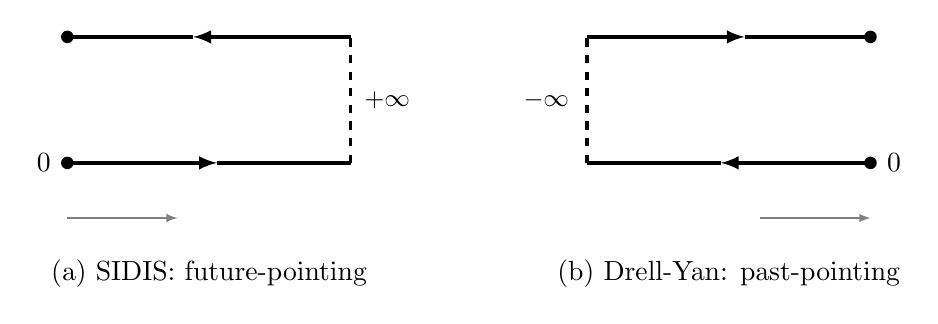
\begin{tikzpicture}[scale=1.0,
    q/.style={circle, fill=black, inner sep=1.6pt}]
  % SIDIS staple
  \begin{scope}[shift={(0,0)}]
    \node[q, label=left:{$0$}] at (0,0) {};
    \node[q, label=left:{$\bvec$}] at (0,1.6) {};
    \draw[very thick, -latex] (0,0) -- (1.9,0);
    \draw[very thick] (1.9,0) -- (3.6,0);
    \draw[very thick, dashed] (3.6,0) -- (3.6,1.6);
    \draw[very thick, -latex] (3.6,1.6) -- (1.6,1.6);
    \draw[very thick] (1.6,1.6) -- (0,1.6);
    \node[right] at (3.65,0.8) {\small $+\infty\,\nminus$};
    \draw[-latex, gray] (0,-0.7) -- (1.4,-0.7) node[right, black] {\small $\nminus$};
    \node at (1.8,-1.4) {(a) SIDIS: future-pointing};
  \end{scope}
  % DY staple
  \begin{scope}[shift={(10.2,0)}]
    \node[q, label=right:{$0$}] at (0,0) {};
    \node[q, label=right:{$\bvec$}] at (0,1.6) {};
    \draw[very thick, -latex] (0,0) -- (-1.9,0);
    \draw[very thick] (-1.9,0) -- (-3.6,0);
    \draw[very thick, dashed] (-3.6,0) -- (-3.6,1.6);
    \draw[very thick, -latex] (-3.6,1.6) -- (-1.6,1.6);
    \draw[very thick] (-1.6,1.6) -- (0,1.6);
    \node[left] at (-3.65,0.8) {\small $-\infty\,\nminus$};
    \draw[-latex, gray] (-1.4,-0.7) -- (0,-0.7) node[right, black] {\small $\nminus$};
    \node at (-1.8,-1.4) {(b) Drell-Yan: past-pointing};
  \end{scope}
\end{tikzpicture}
\caption{Staple-shaped gauge links connecting the quark fields at $0$ and $\bvec$ in the TMD correlator, Eq.~\eqref{eq:tmd_correlator_simple}. (a) In SIDIS the link runs to $+\infty$ along the light-cone direction $\nminus$ of the outgoing quark, Eq.~\eqref{eq:staple_sidis}. (b) In Drell-Yan it runs to $-\infty$, Eq.~\eqref{eq:staple_dy}. The dashed segment is the transverse link at infinity. In the lattice calculation the legs have finite length $\eta|v|$ along a space-like direction $v$, and the two cases correspond to $\eta v\tcdot P\to+\infty$ and $\eta v\tcdot P\to-\infty$ \cite{Musch:2011er}.}
\label{fig:staple_links}
\end{figure}

\subsubsection{Leading-twist TMDs}

At leading twist, the correlator is projected with the Dirac structures $\Gamma = \gamma^+$, $\gamma^+\gamma_5$ and $i\sigma^{i+}\gamma_5$, which select the ``good'' light-cone components of the quark field. Parity, hermiticity and Lorentz covariance then allow eight functions of $x$ and $\vprp{k}^2$ \cite{Ralston:1979ys,Tangerman:1994eh,Mulders:1995dh,Boer:1997nt,Goeke:2005hb}:
\begin{align}
  \Phi^{[\gamma^+]} &= f_1 - \toddmark{\frac{\epsilon_{ij}\,k_{T,i}\,S_{T,j}}{\mN}\,f_{1T}^\perp} \ , \label{eq:tmd_decomp_f}\\
  \Phi^{[\gamma^+\gamma_5]} &= \Lambda\, g_1 + \frac{\vprp{k}\tcdot\vprp{S}}{\mN}\,g_{1T} \ , \label{eq:tmd_decomp_g}\\
  \Phi^{[i\sigma^{i+}\gamma_5]} &= S_{T,i}\,h_1 + \frac{\Lambda\,k_{T,i}}{\mN}\,h_{1L}^\perp - \frac{\left(k_{T,i}k_{T,j} - \frac{1}{2}\vprp{k}^2\delta_{ij}\right)S_{T,j}}{\mN^2}\,h_{1T}^\perp + \toddmark{\frac{\epsilon_{ij}\,k_{T,j}}{\mN}\,h_1^\perp} \ . \label{eq:tmd_decomp_h}
\end{align}
The eight functions are summarized in Table~\ref{tab:leading_twist_tmds}. Three of them survive integration over $\vprp{k}$ and have collinear counterparts: the unpolarized distribution $f_1$, the helicity distribution $g_1$ and the transversity distribution $h_1$. The other five exist only because of the transverse momentum. The worm-gear functions $g_{1T}$ and $h_{1L}^\perp$ and the pretzelosity $h_{1T}^\perp$ correlate the quark transverse momentum with the quark and nucleon polarizations. The Sivers function $f_{1T}^\perp$ and the Boer-Mulders function $h_1^\perp$, marked by the brackets $[\ \ ]_{\text{odd}}$, are the naively T-odd functions.

\begin{table}[htpb]
\centering
\renewcommand{\arraystretch}{1.5}
\begin{tabular}{c|ccc}
  \hline
  nucleon $\backslash$ quark & U & L & T \\
  \hline
  U & $f_1$ & & $\left[h_1^\perp\right]_{\text{odd}}$ \\
  L & & $g_1$ & $h_{1L}^\perp$ \\
  T & $\left[f_{1T}^\perp\right]_{\text{odd}}$ & $g_{1T}$ & $h_1,\ h_{1T}^\perp$ \\
  \hline
\end{tabular}
\caption{Leading-twist quark TMDs, arranged by the polarization of the nucleon (rows) and of the quark (columns): unpolarized (U), longitudinally polarized (L) and transversely polarized (T). The Sivers function $f_{1T}^\perp$ and the Boer-Mulders function $h_1^\perp$ are naively T-odd.}
\label{tab:leading_twist_tmds}
\end{table}

The $\gamma^+$ projection has a density interpretation. In light-cone gauge, $\Phi^{[\gamma^+]}(x,\vprp{k};P,S)$ counts quarks with momentum fraction $x$ and transverse momentum $\vprp{k}$ in a nucleon with spin $S$, summed over quark helicities \cite{CollinsBook2011,Collins:2003fm}. Eq.~\eqref{eq:tmd_decomp_f} is therefore the density of Eq.~\eqref{eq:intro_sivers_density}. Positivity of this density implies the bound $(|\vprp{k}|/\mN)\,|f_{1T}^\perp(x,\vprp{k}^2)| \le f_1(x,\vprp{k}^2)$ \cite{Bacchetta:1999kz}.

\subsubsection{Time reversal and the sign change}

Time reversal is a symmetry of QCD, but it also acts on the gauge link. Combined with parity, it maps the correlator with a future-pointing staple onto the correlator with a past-pointing staple, $\nminus\to-\nminus$ \cite{Collins:2002kn,Boer:2003cm}. Under this map the T-even functions are unchanged, whereas the terms in brackets in Eqs.~\eqref{eq:tmd_decomp_f} and \eqref{eq:tmd_decomp_h} change sign. Combined with the link directions of Eqs.~\eqref{eq:staple_sidis} and \eqref{eq:staple_dy}, this gives
\begin{equation}
  f_{1T}^\perp\big|_{\text{SIDIS}} = -f_{1T}^\perp\big|_{\text{DY}}\ ,\qquad
  h_{1}^\perp\big|_{\text{SIDIS}} = -h_{1}^\perp\big|_{\text{DY}}\ ,\qquad
  f^{\text{T-even}}\big|_{\text{SIDIS}} = f^{\text{T-even}}\big|_{\text{DY}} \ .
  \label{eq:sign_change_all}
\end{equation}
Collins's 1993 argument \cite{Collins:1992kk} used a straight gauge link, which is invariant under time reversal. With such a link the T-odd functions do vanish. The Sivers function is nonzero only because the physical gauge link extends to infinity in a direction set by the process.

The same structure appears in the lattice calculation. The staple of Eq.~\eqref{eq-staplelink} has finite legs of length $\eta|v|$ along a direction $v$, and the SIDIS and DY cases correspond to $\eta v\tcdot P \to +\infty$ and $\eta v\tcdot P\to -\infty$ \cite{Musch:2011er}. T-even quantities are even functions of $\eta$, T-odd quantities are odd, and T-odd quantities vanish for a straight link, $\eta = 0$. The symmetry constraints on the correlator that lead to these statements are worked out in Chapter~\ref{sec:tmd_framework}.

\subsection{Rapidity divergences, the soft factor and evolution}
\label{sec:rapidity_soft}

The staple-shaped links of Eqs.~\eqref{eq:staple_sidis} and \eqref{eq:staple_dy} cause a problem that does not arise for collinear PDFs. Wilson lines along an exactly light-like direction produce divergences from gluons with large rapidity, moving parallel to the Wilson line, which are not regulated by dimensional regularization \cite{Collins:2003fm,Collins:2007ph,CollinsBook2011}. These rapidity divergences cancel in the cross section, between the TMDs and a soft factor, but they have to be regulated in the definition of each TMD.

Collins and Soper introduced the regulator used in this work \cite{Collins:1981uk,Collins:1981uw}: the Wilson lines are tilted away from the light cone into a space-like direction $v$. The approach to the light cone is measured by the Lorentz-invariant parameter
\begin{equation}
  \zetahat = \frac{v\tcdot P}{\sqrt{|v^2|}\,\sqrt{P^2}} = \sinh(y_P - y_v) \ ,
\end{equation}
Eq.~\eqref{eq-zeta}, where $y_P$ and $y_v$ are the rapidities of $P$ and $v$. The light-cone limit is $\zetahat\to\infty$. A space-like $v$ has an important advantage for the lattice: one can always boost to a frame in which $v$ has no time component, so that the entire operator lies at a single time \cite{Musch:2011er,Aybat:2011zv}.

The soft factor $\tilde{\softf}$ is a vacuum expectation value of Wilson lines, essentially a Wilson loop made from two staples. Dividing the unsubtracted correlator by an appropriate combination of soft factors, Eq.~\eqref{eq-corr}, removes the rapidity divergences and the dependence on the regulator in the limit where the Wilson lines approach the light cone \cite{CollinsBook2011,Aybat:2011zv}. The Wilson lines also have a self-energy that diverges linearly with the ultraviolet cutoff, proportional to the length of the path. On the lattice this divergence appears as a factor $e^{-\delta m\, L}$ for a path of length $L$, with $\delta m\propto 1/a$, together with additional divergences from the corners of the path \cite{MuschThesis2,Musch:2010ka}. For a fixed path, both the soft factor and these renormalization factors multiply the correlator independently of the Dirac structure $\Gamma$ \cite{Musch:2011er}. They therefore cancel in ratios of amplitudes taken at the same $\bvec$, $P$ and staple geometry. The observables computed in this thesis are ratios of this type.

After the rapidity divergences are removed, the TMDs depend on two scales: the renormalization scale $\mu$ and the rapidity scale $\zeta$. In the convention of Collins, the dependence on them is described by the Collins-Soper equations \cite{Collins:1981uk,Collins:1984kg,CollinsBook2011},
\begin{equation}
  \frac{\partial\ln\tilde{f}(x,\vprp{b};\mu,\zeta)}{\partial\ln\sqrt{\zeta}} = \tilde{K}(|\vprp{b}|;\mu) \ ,\qquad
  \frac{d\tilde{K}(|\vprp{b}|;\mu)}{d\ln\mu} = -\gamma_K\big(\alpha_s(\mu)\big) \ ,
  \label{eq:cs_equation}
\end{equation}
together with a renormalization group equation in $\mu$. The Collins-Soper kernel $\tilde K$ is independent of $x$ and of the hadron, and $\gamma_K$ is the cusp anomalous dimension. For $|\vprp{b}|\lesssim 1/\Lambda_{\text{QCD}}$ the kernel can be computed in perturbation theory. At larger $|\vprp{b}|$ it is non-perturbative, and it is one of the quantities that recent lattice calculations have determined \cite{Ebert:2018gzl,Shanahan:2021tst,Schlemmer:2021aij,LatticePartonLPC:2022eev}. The evolution of the Sivers function in these scales has been worked out in Refs.~\cite{Aybat:2011ge,Echevarria:2014xaa}. In the lattice calculation the scale $\zeta$ is represented by $\zetahat$, which is finite at accessible nucleon momenta, and the light-cone limit has to be reached by extrapolation (Chapter~\ref{sec:physical_limit_extrapolation}).

\subsection{Transverse position space and the Sivers shift}
\label{sec:bt_space_sivers_shift}

Lattice calculations produce matrix elements at fixed separations $\bvec$, so it is natural to work with TMDs in transverse position space. The Fourier transform $\tilde f(x,\vprp{b}^2)$ and its derivatives $\tilde f^{(n)}(x,\vprp{b}^2)$ with respect to $\vprp{b}^2$ are defined in Eqs.~\eqref{eq-FTMD} and \eqref{eq-dFTMD}. As $|\vprp{b}|\to 0$ they reduce to the transverse momentum moments
\begin{equation}
  f^{(n)}(x) = \int d^2\vprp{k}\left(\frac{\vprp{k}^2}{2\mN^2}\right)^n f(x,\vprp{k}^2) \ ,
\end{equation}
Eq.~\eqref{eq-btder2}. For the Sivers function, the first moment $f_{1T}^{\perp(1)}(x)$ is the quantity that enters the transverse momentum weighted Sivers asymmetry. It is also ultraviolet divergent in QCD, because the perturbative large-$\vprp{k}$ tail of the Sivers function falls off too slowly \cite{Bacchetta:2008xw}. A finite $|\vprp{b}|$ acts as a regulator, and we keep $|\vprp{b}|$ finite throughout \cite{Musch:2011er,Boer:2011xd}. We also use the notation $f^{[m]}$ for $x$-moments, $f^{[1]} = \int_{-1}^{1}dx\, f(x)$.

In $\vprp{b}$ space, the $\gamma^+$ projection of the correlator contains two Lorentz-invariant amplitudes \cite{Musch:2011er},
\begin{equation}
  \frac{1}{2P^+}\,\tilde\Phi^{[\gamma^+]}_{\unsub} = \tAmp_{2B} + i\mN\,\epsilon_{ij}\,b_i\,S_j\ \tAmp_{12B} \ ,
  \label{eq:gamma_plus_amplitudes}
\end{equation}
where $\tAmp_{2B}$ gives the unpolarized TMD and $\tAmp_{12B}$ the Sivers function after the Fourier transform in $\bvec\tcdot P$ and division by the soft factor. Their definitions in terms of the full set of invariant amplitudes are given in Eq.~\eqref{eq-ABamps_sivers}. At $\bvec\tcdot P = 0$ the Fourier transform in $\bvec\tcdot P$ reduces to an integral over $x$, and one finds \cite{Musch:2011er}
\begin{equation}
  \tilde f_1^{[1](0)}(\vprp{b}^2) = \frac{2\tAmp_{2B}}{\tilde{\softf}}\ ,\qquad
  \tilde f_{1T}^{\perp[1](1)}(\vprp{b}^2) = -\frac{2\tAmp_{12B}}{\tilde{\softf}}\ ,
\end{equation}
with both amplitudes evaluated at $\bvec^2 = -\vprp{b}^2$ and $\bvec\tcdot P = 0$.

The Sivers function describes the average transverse momentum of unpolarized quarks in the direction perpendicular to the nucleon spin. For a nucleon polarized along $\hat{\vect{x}}$, $\vprp{S} = (1,0)$, Eq.~\eqref{eq:tmd_decomp_f} gives $\Phi^{[\gamma^+]} = f_1 + (k_y/\mN)\,f_{1T}^\perp$, and the average $k_y$ is $\mN f_{1T}^{\perp(1)}/f_1^{(0)}$. The generalized Sivers shift extends this quantity to finite $|\vprp{b}|$ \cite{Musch:2011er,Boer:2011xd},
\begin{equation}
  \langle k_y\rangle_{TU}(\vprp{b}^2;\zetahat,\eta v\tcdot P) \equiv \mN\,\frac{\tilde f_{1T}^{\perp[1](1)}(\vprp{b}^2;\zetahat,\ldots,\eta v\tcdot P)}{\tilde f_1^{[1](0)}(\vprp{b}^2;\zetahat,\ldots,\eta v\tcdot P)}
  = -\mN\,\frac{\tAmp_{12B}(-\vprp{b}^2,0,0,-1/(\mN\zetahat)^2,\eta v\tcdot P)}{\tAmp_{2B}(-\vprp{b}^2,0,0,-1/(\mN\zetahat)^2,\eta v\tcdot P)} \ .
  \label{eq:generalized_sivers_shift}
\end{equation}
The soft factor and the multiplicative renormalization factors cancel in the ratio, so $\langle k_y\rangle_{TU}$ can be computed on the lattice without constructing either. In the limit $|\vprp{b}|\to 0$ it would become the average transverse momentum of the quarks, with the numerator summing quark and antiquark contributions and the denominator counting quarks minus antiquarks \cite{Boussarie:2023izj}. Because $\bvec\tcdot P = 0$, Eq.~\eqref{eq:generalized_sivers_shift} is integrated over $x$.

The $x$ dependence enters through the second argument of the amplitudes. Since $x$ and $\bvec\tcdot P$ are Fourier conjugate variables (Chapter~\ref{sec:tmd_framework}), keeping $\bvec\tcdot P$ as a variable and Fourier transforming the numerator and denominator separately gives an $x$-dependent generalized Sivers shift,
\begin{equation}
  \langle k_y\rangle_{TU}(x,\vprp{b}^2;\zetahat,\eta v\tcdot P) = -\mN\,\frac{\int d(\bvec\tcdot P)\ e^{ix(\bvec\tcdot P)}\ \tAmp_{12B}(\bvec^2,\bvec\tcdot P,\ldots)}{\int d(\bvec\tcdot P)\ e^{ix(\bvec\tcdot P)}\ \tAmp_{2B}(\bvec^2,\bvec\tcdot P,\ldots)} \ .
\end{equation}
The soft factor depends only on $\vprp{b}$, not on $\bvec\tcdot P$, so it still cancels \cite{Boussarie:2023izj}. This is the quantity computed in this thesis. The full expression, including the kinematic constraint that relates $v\tcdot\bvec$ to $\bvec\tcdot P$, is Eq.~\eqref{eq:sivers_shift_xdep} in Chapter~\ref{sec:x_dependence}.

\subsection{From \texorpdfstring{$\bvec\tcdot P$}{b.P} to \texorpdfstring{$x$}{x}}
\label{sec:bP_to_x}

Because the $x$ dependence is obtained through a Fourier transform, it is useful to state what the $\bvec\tcdot P$ dependence of an amplitude tells us about the corresponding distribution. We take the unpolarized case as the example. At fixed $\bvec^2 = -\vprp{b}^2$, the relation $f_1 = 2\fourint\tAmp_{2B}$ of Eq.~\eqref{eq-tmdsfromampsodd} can be inverted in the longitudinal variable. Since $\tilde f_1(x,\vprp{b}^2)$ vanishes outside $-1\le x\le 1$,
\begin{equation}
  \tAmp_{2B}(-\vprp{b}^2,\bvec\tcdot P) = \frac{\tilde{\softf}}{2}\int_{-1}^{1}dx\ e^{-ix(\bvec\tcdot P)}\ \tilde f_1(x,\vprp{b}^2) \ ,
  \label{eq:amplitude_from_tmd}
\end{equation}
where we have suppressed the remaining arguments of the amplitude and of the soft factor. Three properties follow directly from this representation.

First, the Taylor coefficients of the amplitude in $\bvec\tcdot P$ are the Mellin moments of the distribution at fixed $\vprp{b}$,
\begin{equation}
  \frac{\tAmp_{2B}(-\vprp{b}^2,\bvec\tcdot P)}{\tAmp_{2B}(-\vprp{b}^2,0)} = \sum_{n=0}^{\infty}\frac{(-i\,\bvec\tcdot P)^n}{n!}\ \langle x^n\rangle_{\vprp{b}} \ ,\qquad
  \langle x^n\rangle_{\vprp{b}} = \frac{\int dx\,x^n\,\tilde f_1(x,\vprp{b}^2)}{\int dx\,\tilde f_1(x,\vprp{b}^2)} \ .
  \label{eq:taylor_moments}
\end{equation}
The value at $\bvec\tcdot P = 0$ is the $x$-integrated quantity studied in earlier work, and the first few derivatives give low moments of the kind that local operators provide. Musch used this relation with straight links to estimate the lowest moments of the unpolarized distribution \cite{MuschThesis2}.

Second, the real and imaginary parts of the amplitude separate quark and antiquark contributions. Using $f_1^{\bar q}(x) = -f_1^q(-x)$ for $x>0$, and taking the soft factor to be real,
\begin{align}
  \myRe\,\tAmp_{2B} &= \frac{\tilde{\softf}}{2}\int_0^1 dx\ \cos\big(x\,\bvec\tcdot P\big)\left[\tilde f_1^q(x) - \tilde f_1^{\bar q}(x)\right] , \nonumber\\
  \myIm\,\tAmp_{2B} &= -\frac{\tilde{\softf}}{2}\int_0^1 dx\ \sin\big(x\,\bvec\tcdot P\big)\left[\tilde f_1^q(x) + \tilde f_1^{\bar q}(x)\right] .
  \label{eq:re_im_valence}
\end{align}
The real part, which is even in $\bvec\tcdot P$, is determined by the quark-minus-antiquark (valence-like) combination, and the imaginary part, which is odd, by the quark-plus-antiquark combination. This is the parity structure used in Chapter~\ref{sec:x_dependence}. For the naively T-odd Sivers function the antiquark enters with the opposite relative sign \cite{Boussarie:2023izj}, so the roles of the two combinations are interchanged for $\tAmp_{12B}$.

Third, the support property constrains how the amplitude can behave at large $|\bvec\tcdot P|$. If $\tilde f_1$ is integrable, the Riemann-Lebesgue lemma implies $\tAmp_{2B}\to 0$ as $|\bvec\tcdot P|\to\infty$, and since the support is bounded, $\tAmp_{2B}$ extends to an entire function of $\bvec\tcdot P$ of exponential type no larger than one. A parametrization of lattice data that grows with $|\bvec\tcdot P|$ at fixed $\bvec^2$ is therefore inconsistent with a physical distribution and has no Fourier transform in the ordinary sense. This criterion is used in Section~\ref{sec:gaussian_transformation} to reject the Gaussian ansatz. A parametrization that decays like a power of $\bvec\tcdot P$ fast enough to be absolutely integrable does have a Fourier transform. It is in general not an entire function, so the resulting distribution is not guaranteed to vanish outside $|x|\le 1$, and the size of any such tail is one measure of the model dependence.

Lattice data cover only a finite range of $\bvec\tcdot P$, because $|\bvec\tcdot P|\le |\vect{P}|\,|\vect{b}|$ in a frame where $\bvec$ has no time component (Section~\ref{sec:tmds_lattice_approaches}). The behavior of $\tilde f$ at small $|x|$ is governed by the amplitude at large $|\bvec\tcdot P|$, outside the range of the data. The $x$ dependence reconstructed from a finite range of $\bvec\tcdot P$ therefore depends on the functional form used to describe the data, and it depends on it most strongly at small $x$. This is why the choice and validation of fit models take up a large part of this thesis (Chapter~\ref{sec:fitting_methodologies}).

\subsection{TMDs from lattice QCD}
\label{sec:tmds_lattice_approaches}

Lattice QCD works in Euclidean space-time. A non-local operator can be evaluated directly only if all of its points lie at a single Euclidean time, which corresponds to purely space-like separations in Minkowski space. Operators that extend along a light-like direction, like those in Eq.~\eqref{eq:collinear_pdf} and Eq.~\eqref{eq:tmd_correlator_simple}, cannot be placed on the lattice as they stand. Three strategies have been developed to deal with this.

The first is the local operator approach of Section~\ref{sec:dis}. Mellin moments are matrix elements of local operators and are computed directly, but only the lowest moments are accessible. For TMDs this approach does not apply at all, because the staple-shaped link cannot be expanded into local operators.

The second is the Lorentz-invariant amplitude approach of Musch, H\"agler, Engelhardt, Negele and Sch\"afer \cite{Hagler:2009mb,Musch:2010ka,Musch:2011er}, used in this thesis. The correlator with a finite, space-like staple is decomposed into amplitudes $\tAmp_i$ and $\tBmp_i$ that depend only on Lorentz invariants: $\bvec^2$, $\bvec\tcdot P$, $\zetahat$ and the staple length through $\eta v\tcdot P$ \cite{Goeke:2005hb}. Because $\bvec$ and $v$ are space-like, there is a frame in which both have vanishing time components, and in that frame the operator can be evaluated at a single Euclidean time. The amplitudes computed there are, by Lorentz invariance, the same amplitudes that define TMDs in the light-cone frame. The accessible kinematics are limited by the lattice. In a frame with $b^0 = v^0 = 0$, the invariants become $\bvec\tcdot P = -\vect{b}\tcdot\vect{P}$ and $\zetahat = -\vect{v}\tcdot\vect{P}/(|\vect{v}|\,\mN)$, so that
\begin{equation}
  |\bvec\tcdot P| \le |\vect{P}|\,|\vect{b}|\ ,\qquad |\zetahat| \le \frac{|\vect{P}|}{\mN} \ .
\end{equation}
Nonzero $\bvec\tcdot P$ requires a component of $\vect{b}$ along the nucleon momentum, and large $\zetahat$ requires large nucleon momenta, where the statistical signal deteriorates. The light-cone limit $\zetahat\to\infty$ and the SIDIS and DY limits $\eta v\tcdot P\to\pm\infty$ are reached by extrapolation. Soft factors and renormalization constants cancel in the ratios discussed in Section~\ref{sec:bt_space_sivers_shift}. With this approach the Sivers and Boer-Mulders shifts, the worm-gear shift and the generalized tensor charge have been computed for the nucleon and the pion \cite{Musch:2011er,Engelhardt:2015xja,Yoon:2015ocs,Yoon:2017qzo}.

The third strategy is large-momentum effective theory (LaMET) \cite{Ji:2013dva,Ji:2020ect}. Instead of Lorentz invariance, it uses the fact that an equal-time correlator in a hadron with large momentum $P^z$ approaches the light-cone correlator, up to a perturbative matching and corrections suppressed by powers of $1/P^z$. For TMDs, the quasi-TMD is defined with a staple along the $z$ direction and a Fourier transform in the longitudinal separation, and it is related to the light-cone TMD by a matching coefficient, a factor involving the Collins-Soper kernel, and a reduced soft function that can itself be computed on the lattice \cite{Ji:2014hxa,Ebert:2018gzl,Ji:2019sxk,Ebert:2022fmh}. Ratios of quasi-TMDs at different momenta give the Collins-Soper kernel \cite{Ebert:2018gzl,Shanahan:2021tst,LatticePartonLPC:2022eev}. A related approach uses pseudo-distributions, which are functions of the Lorentz invariants $\bvec\tcdot P$ and $\bvec^2$ \cite{Radyushkin:2017cyf}. For infinitely long staples, the Lorentz-invariant and LaMET definitions of the beam function coincide, and both can be matched to the continuum TMDs \cite{Ebert:2022fmh}. Reviews of these methods can be found in Refs.~\cite{Lin:2017snn,Constantinou:2020hdm,Boussarie:2023izj}.

The Lorentz-invariant approach is well suited to ratio observables such as the Sivers shift, because it works directly with the amplitudes in which soft factors cancel and it makes the dependence on $\bvec\tcdot P$ explicit. That dependence is what this thesis uses to reach the $x$ dependence. The next chapter describes how the correlation functions are computed on the lattice.
